\section{Force Field Parameters}
\label{section:forcefield}


\subsection{Potential energy functions}

Evaluating the force is the most computationally demanding
part of molecular dynamics.
The force is the negative gradient of a scalar potential energy function,
\begin{equation}
\vec{F}(\vec{r}) = -\nabla U(\vec{r}),
\end{equation}
and, for systems of biomolecules,
this potential function involves the summing,
\begin{equation}
U(\vec{r}) = \sum U_{\text{bonded}}(\vec{r})
  + \sum U_{\text{nonbonded}}(\vec{r}),
\end{equation}
over a large number of bonded and nonbonded terms.
The bonded potential terms involve 2--, 3--, and 4--body interactions
of covalently bonded atoms,
with $O(N)$ terms in the summation.
The nonbonded potential terms involve interactions
between all pairs of atoms
(usually excluding pairs of atoms already involved in a bonded term),
with $O(N^2)$ terms in the summation,
although fast evaluation techniques are used to
compute good approximations to their contribution to the potential
with $O(N)$ or $O(N \log N)$ computational cost.


\subsubsection{Bonded potential energy terms}
%\label{sec:bonded}

The bonded potential terms involve 2--, 3--, and 4--body interactions
of covalently bonded atoms.

The 2--body spring bond potential
describes the harmonic vibrational motion
between an $(i,j)$--pair of covalently bonded atoms,
\begin{equation}
U_{\text{bond}} = k (r_{ij} - r_0)^2,
\end{equation}
where $r_{ij} = \|\vec{r}_j - \vec{r}_i\|$ gives the distance
between the atoms,
$r_0$ is the equilibrium distance,
and $k$ is the spring constant.

The 3--body angular bond potential
describes the angular vibrational motion
occurring between an $(i,j,k)$--triple of covalently bonded atoms,
\begin{equation}
U_{\text{angle}} = k_{\theta} (\theta - \theta_0)^2
                 + k_{\text{ub}} (r_{ik} - r_{\text{ub}})^2,
\end{equation}
where, in the first term,
$\theta$ is the angle in radians between vectors
$\vec{r}_{ij} = \vec{r}_j - \vec{r}_i$
and $\vec{r}_{kj} = \vec{r}_j - \vec{r}_k$,
$\theta_0$ is the equilibrium angle,
and $k_{\theta}$ is the angle constant.
The second term is the Urey--Bradley term
used to describe a 
(noncovalent) spring between the outer $i$ and $k$ atoms,
active when constant $k_{\text{ub}} \neq 0$,
where, like the spring bond,
$r_{ik} = \|\vec{r}_k - \vec{r}_i\|$ gives the distance between
the pair of atoms and
$r_{\text{ub}}$ is the equilibrium distance.

The 4--body torsion angle (also known as dihedral angle) potential
describes the angular spring between the planes formed
by the first three and last three atoms of
a consecutively bonded $(i,j,k,l)$--quadruple of atoms,
\begin{equation}
U_{\text{tors}} =
  \begin{cases}
  k (1 + \cos(n \psi + \phi)) & \text{if $n > 0$,} \\
  k (\psi - \phi)^2           & \text{if $n = 0$,}
  \end{cases}
\end{equation}
where $\psi$ is the angle in radians between
the $(i,j,k)$--plane and the $(j,k,l)$--plane.
The integer constant $n$ is nonnegative and indicates the periodicity.
For $n > 0$, $\phi$ is the phase shift angle
and $k$ is the multiplicative constant.
For $n = 0$, $\phi$ acts as an equilibrium angle
and the units of $k$ change to $\text{potential}/\text{rad}^2$.
A given $(i,j,k,l)$--quadruple of atoms might contribute
multiple terms to the potential,
each with its own parameterization.
The use of multiple terms for a torsion angle allows for
complex angular variation of the potential,
effectively a truncated Fourier series.


\subsubsection{Nonbonded potential energy terms}
%\label{sec:nonbonded}

The nonbonded potential terms involve interactions
between all $(i,j)$--pairs of atoms,
usually excluding pairs of atoms already involved in a bonded term.
Even using a fast evaluation methods
the cost of computing the nonbonded potentials dominates the work
required for each time step of an MD simulation.

The Lennard--Jones potential
accounts for the weak dipole attraction between distant atoms and
the hard core repulsion as atoms become close,
\begin{equation}
U_{\text{LJ}} = (-E_{\text{min}}) \left[ 
    \left( \frac{R_{\text{min}}}{r_{ij}} \right)^{12} -
    2 \left( \frac{R_{\text{min}}}{r_{ij}} \right)^{6} \right],
\end{equation}
where $r_{ij} = \|\vec{r}_j - \vec{r}_i\|$ gives the distance
between the pair of atoms.
The parameter $E_{\text{min}} = U_{\text{LJ}}(R_{\text{min}})$ is 
the minimum of the potential term
($E_{\text{min}} < 0$, which means that $-E_{\text{min}}$ is the well-depth).
The Lennard--Jones potential approaches 0 rapidly as $r_{ij}$
increases, so it is usually truncated (smoothly shifted) to 0
past a cutoff radius, requiring $O(N)$ computational cost.

The electrostatic potential
is repulsive for atomic charges with the same sign
and attractive for atomic charges with opposite signs,
\begin{equation}
U_{\text{elec}} = \epsilon_{14} \frac{C q_i q_j}{\epsilon_0 r_{ij}},
\end{equation}
where $r_{ij} = \|\vec{r}_j - \vec{r}_i\|$ gives the distance
between the pair of atoms,
and $q_i$ and $q_j$ are the charges on the respective atoms.
Coulomb's constant $C$ and the dielectric constant $\epsilon_0$
are fixed for all electrostatic interactions.
The parameter $\epsilon_{14}$ is a unitless scaling factor 
whose value is 1,
except for a modified 1--4 interaction,
where the pair of atoms is separated by a sequence
of three covalent bonds (so that the atoms might
also be involved in a torsion angle interaction),
in which case $\epsilon_{14} = \varepsilon$,
for a fixed constant $0 \leq \varepsilon \leq 1$.
Although the electrostatic potential may be computed with
a cutoff like the Lennard--Jones potential,
the $1/r$ potential approaches 0 much more
slowly than the $1/r^6$ potential,
so neglecting the long range electrostatic terms
can degrade qualitative results,
especially for highly charged systems.
There are other fast evaluation methods that approximate
the contribution to the long range electrostatic terms
that require $O(N)$ or $O(N \log N)$ computational cost,
depending on the method.


\subsection{Non-bonded interactions}
\label{section:electdesc}

\NAMD\ has a number of options that control the way that non-bonded
interactions are calculated.  These options are interrelated and
can be quite confusing, so this section attempts to explain the
behavior of the non-bonded interactions and how to use these
parameters.

\subsubsection{Van der Waals interactions}
The simplest non-bonded 
interaction is the van der Waals interaction.  In 
\NAMD, van der Waals interactions are always truncated at the 
cutoff distance, specified by {\tt cutoff}.  
The main option that effects van der Waals interactions
is the {\tt switching} parameter.  With this option set to {\tt on},
a smooth switching function will be used to truncate the
van der Waals potential energy smoothly at the cutoff distance.  
A graph of the van der Waals 
potential with this switching function is shown in Figure 
\ref{fig:switching}.  If {\tt switching} is set to {\tt off}, the 
van der Waals energy is just abruptly truncated at the cutoff 
distance, so that energy may not be conserved.  

\begin{figure}[htb]
  \center{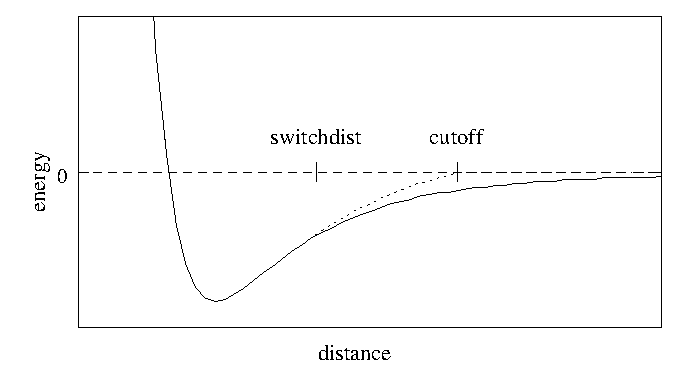
\includegraphics{figures/switching}}
  \caption[Graph of van der Waals potential with and without switching]
  {\small Graph of van der Waals potential with and without the
  application of the switching function.  With the switching function
  active, the potential is smoothly reduced to 0 at the cutoff distance.
  Without the switching function, there is a discontinuity where the
  potential is truncated.}
  \label{fig:switching}
\end{figure}

The switching function used is based on the X-PLOR switching
function.  The parameter {\tt switchdist} specifies the distance
at which the switching function should start taking effect to
bring the van der Waals potential to 0 smoothly at the cutoff distance.  
Thus, the value of {\tt switchdist} must always be less than that 
of {\tt cutoff}.


\subsubsection{Electrostatic interactions}
The handling of electrostatics is slightly
more complicated due to the incorporation of multiple timestepping for full
electrostatic interactions.  There are two cases to consider, one where
full electrostatics is employed and the other where electrostatics
are truncated at a given distance.
\prettypar
First let us consider the latter case, where electrostatics are truncated at
the cutoff distance.  Using this scheme, all electrostatic interactions
beyond a specified distance are ignored, or assumed to be zero.  If
{\tt switching} is set to {\tt on}, rather than having a discontinuity
in the potential
at the cutoff distance, a shifting function is applied to the electrostatic
potential as shown in Figure \ref{fig:shifting}.  As this figure shows, the
shifting function shifts the entire potential curve so that the curve
intersects the x-axis at the cutoff distance.  This shifting function
is based on the
shifting function used by X-PLOR.

\begin{figure}[htb]
  \center{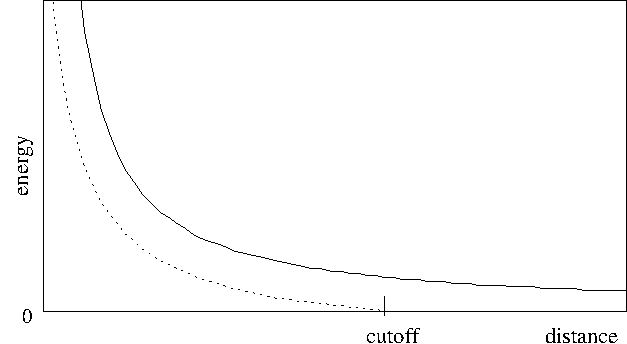
\includegraphics{figures/shifting}}
  \caption[Graph of electrostatic potential with and without shifting function]
  {\small Graph showing an electrostatic potential with and without the
  application of the shifting function.}
  \label{fig:shifting}
\end{figure}

Next, consider the case where full electrostatics are calculated.  In this
case, the electrostatic interactions are not truncated at any distance.  In
this scheme, the {\tt cutoff} parameter has a slightly different meaning
for the electrostatic interactions --- it represents
the {\it local interaction distance\/}, or distance within which electrostatic
pairs will be directly calculated every timestep.  Outside of this distance,
interactions will be calculated only periodically.  These forces
will be applied using a multiple timestep integration scheme as described in
Section \ref{section:mts}.

\begin{figure}[htb]
  \center{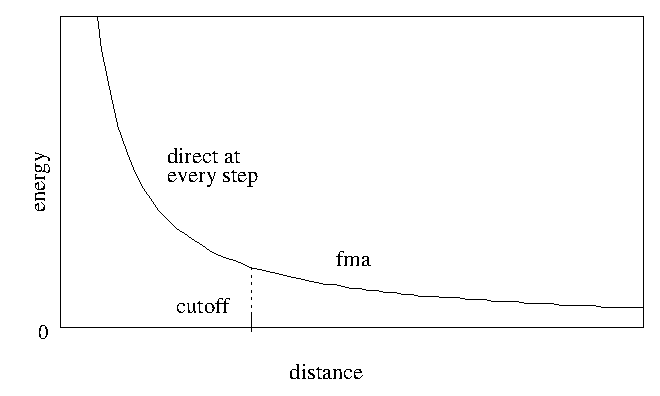
\includegraphics{figures/fmaOn}}
  \caption[Graph of electrostatic split between short and long range forces]
  {\small Graph showing an electrostatic potential 
  when full electrostatics are used within \NAMD, 
  with one curve portion calculated directly 
  and the other calculated using PME.}
  \label{fig:fmaOn}
\end{figure}



\subsubsection{Non-bonded force field parameters}

\begin{itemize}
%\item
%\NAMDCONF{eleccutoff}%
%{local interaction distance for electrostatic calculations (\AA)}%
%{positive decimal}%
%{Specifies the distance at which
%electrostatic interactions are truncated.
%If {\tt eleccutoff} is defined, it supersedes {\tt cutoff}.
%If {\tt eleccutoff} is not defined, then \verb }cutoff} {\em must}
%be defined.
%See Section \ref{section:electdesc} for a further discussion
%of this configuration value.}

%\item
%\NAMDCONF{vdwcutoff}%
%{local interaction distance for van der Waals calculations (\AA)}%
%{positive decimal}%
%{This value specifies the distance at which
%van der Waals interactions are truncated.
%If {\tt vdwcutoff} is defined, it supersedes {\tt cutoff}.
%If {\tt vdwcutoff} is not defined, then \verb }cutoff} {\em must}
%be defined.
%See Section \ref{section:electdesc} for a further discussion
%of this configuration value.}

\item
\NAMDCONF{cutoff}
{local interaction distance common to both electrostatic 
and van der Waals calculations (\AA)}
{positive decimal}
{%This value can substitute for either {\tt eleccutoff}
%or {\tt vdwcutoff} if either of those is undefined.
See Section \ref{section:electdesc} for more information.}

\item
\NAMDCONFWDEF{switching}{use switching function?}{{\tt on} or {\tt off}}
{{\tt on}}
{If {\tt switching} is
specified to be {\tt off}, then a truncated cutoff is performed.
If {\tt switching} is turned {\tt on}, then smoothing functions
are applied to both the electrostatics and van der Waals forces.
For a complete description of the non-bonded force parameters see
Section \ref{section:electdesc}.  If {\tt switching} is set to
{\tt on}, then {\tt switchdist} must also be defined.}

\item
\NAMDCONFWDEF{vdwForceSwitching}{use force switching for VDW?}{{\tt on} or {\tt off}}
{{\tt off}}
{If both {\tt switching} and {\tt vdwForceSwitching} are set to {\tt on},
then CHARMM force switching is used for van der Waals forces.
{\bf LJcorrection as implemented is inconsistent with vdwForceSwitching.}}

%\item
%\NAMDCONF{elecswitchdist}{distance at which to activate switching function for %electrostatic calculations (\AA)}{positive decimal $\leq$ {\tt eleccutoff}}
%{Distance at which the switching function
%used to smooth the truncation of
%electrostatic forces should begin to take effect.  
%This parameter only has meaning if {\tt switching} is 
%set to {\tt on}.  
%The value of {\tt elecswitchdist} must be less than
%or equal to the value of {\tt eleccutoff}, since the switching function
%is only applied on the range from {\tt elecswitchdist} to {\tt eleccutoff}.
%If {\tt elecswitchdist} is defined, it supersedes {\tt switchdist}.
%If {\tt elecswitchdist} is not defined and {\tt switching} is
%{\tt on}, then \verb }switchdist} {\em must} be defined.
%For a complete description of the non-bonded force parameters, see
%Section \ref{section:electdesc}.
%}

%\item
%\NAMDCONF{vdwswitchdist}%
%{distance at which to activate switching function 
%for van der Waals calculations (\AA)}%
%{positive decimal $\leq$ {\tt vdwcutoff}}%
%{Distance at which the switching function
%used to smooth the truncation of
%van der Waals forces should begin to take effect.  
%This parameter only has meaning if {\tt switching} is 
%set to {\tt on}.  
%The value of {\tt vdwswitchdist} must be less than
%or equal to the value of {\tt vdwcutoff}, since the switching function
%is only applied on the range from {\tt vdwswitchdist} to {\tt vdwcutoff}.
%If {\tt vdwswitchdist} is defined, it supersedes {\tt switchdist}.
%If {\tt vdwswitchdist} is not defined and {\tt switching} is
%{\tt on}, then \verb }switchdist} {\em must} be defined.
%For a complete description of the non-bonded force parameters, see
%Section \ref{section:electdesc}.
%}

\item
\NAMDCONF{switchdist}
{distance at which to activate switching/splitting function 
for electrostatic and van der Waals calculations (\AA)}
{positive decimal $\leq$ {\tt cutoff}}
{Distance at which the switching function
should begin to take effect.  
This parameter only has meaning if {\tt switching} is 
set to {\tt on}.  
The value of {\tt switchdist} must be less than
or equal to the value of {\tt cutoff}, since the switching function
is only applied on the range from {\tt switchdist} to {\tt cutoff}.  
For a complete description of the non-bonded force parameters see
Section \ref{section:electdesc}.}

\item
\NAMDCONF{exclude}
{non-bonded exclusion policy to use}
{{\tt none}, {\tt 1-2}, {\tt 1-3}, {\tt 1-4}, or {\tt scaled1-4}}
{\label{param:exclude}
%% This parameter is {\it required\/} for every simulation.
This parameter specifies which pairs of bonded atoms should
be excluded from non-bonded
interactions.  With the value of {\tt none}, no bonded pairs of atoms 
will be excluded.  With the value of {\tt 1-2}, all atom pairs that
are directly connected via a linear bond will be excluded.  With the
value of {\tt 1-3}, all {\tt 1-2} pairs will be excluded along with
all pairs of atoms that are bonded to a common
third atom (i.e., if atom A is bonded to atom B and atom B is bonded
to atom C, then the atom pair A-C would be excluded).
With the value of {\tt 1-4}, all {\tt 1-3} pairs will be excluded along
with all pairs connected by a set of two bonds (i.e., if atom A is bonded
to atom B, and atom B is bonded to atom C, and atom C is bonded to
atom D, then the atom pair A-D would be excluded).  With the value
of {\tt scaled1-4}, all {\tt 1-3} pairs are excluded and all pairs
that match the {\tt 1-4} criteria are modified.  The electrostatic
interactions for such pairs are modified by the constant factor
defined by {\tt 1-4scaling}.  
The van der Waals interactions are modified
by using the special 1-4 parameters defined in the parameter files.
The value of {\tt scaled1-4} is necessary to enable the modified
1-4 VDW parameters present in the CHARMM parameter files.
}

\item
\NAMDCONFWDEF{1-4scaling}{scaling factor for 1-4 electrostatic interactions}
{0 $\leq$ decimal $\leq$ 1}{1.0}
{Scaling factor for 1-4 electrostatic interactions.
This factor is only used when the
{\tt exclude} parameter is set to {\tt scaled1-4}.  In this case, this
factor is used to modify the electrostatic interactions between 1-4 atom
pairs.  If the {\tt exclude} parameter is set to anything but 
{\tt scaled1-4}, this parameter has no effect regardless of its value.}

\item
\NAMDCONFWDEF{dielectric}{dielectric constant for system}
{decimal $\geq$ 1.0}{1.0}
{Dielectric constant for the system.  A value of 1.0 implies no modification
of the electrostatic interactions.  Any larger value will lessen the
electrostatic forces acting in the system.}

\item
\NAMDCONFWDEF{nonbondedScaling}{scaling factor for nonbonded forces}
{decimal $\geq$ 0.0}{1.0}
{Scaling factor for electrostatic and van der Waals forces.
A value of 1.0 implies no modification of the interactions.
Any smaller value will lessen the
nonbonded forces acting in the system.}

\item
\NAMDCONFWDEF{vdwGeometricSigma}{use geometric mean to combine L-J sigmas}
{{\tt yes} or {\tt no}}{{\tt no}}
{Use geometric mean, as required by \index{OPLS} OPLS, rather than
traditional arithmetic mean when combining Lennard-Jones sigma parameters
for different atom types.}

\item
\NAMDCONFWDEF{limitdist}
{maximum distance between pairs for limiting interaction strength(\AA)}
{non-negative decimal}
{{\tt 0.}}
{
The electrostatic and van der Waals potential functions diverge
as the distance between two atoms approaches zero.
The potential for atoms closer than {\tt limitdist} is instead
treated as $a r^2 + c$ with parameters chosen to match the
force and potential at {\tt limitdist}.
This option should primarily be useful for alchemical free energy
perturbation calculations, since it makes the process of creating
and destroying atoms far less drastic energetically.
The larger the value of {\tt limitdist} the more the maximum force
between atoms will be reduced.
In order to not alter the other interactions in the simulation,
{\tt limitdist} should be less than the closest approach
of any non-bonded pair of atoms; 1.3\,\AA\ appears to satisfy this
for typical simulations but the user is encouraged to experiment.
There should be no performance impact from enabling this feature.
}

\item
\NAMDCONFWDEF{LJcorrection}
{Apply long-range corrections to the system energy and virial to
account for neglected vdW forces?}{{\tt yes} or {\tt no}}{{\tt no}}
{Apply an analytical correction to the reported vdW energy and virial
that is equal to the amount lost due to switching and cutoff of the LJ
potential. The correction will use the average of vdW parameters for
all particles in the system and assume a constant, homogeneous
distribution of particles beyond the switching distance. See 
\cite{Shirts2007} for details (the equations used in the NAMD
implementation are slightly different due to the use of a different
switching function). Periodic boundary conditions are required to make
use of tail corrections.
{\bf LJcorrection as implemented is inconsistent with vdwForceSwitching.}}

\end{itemize}


\subsubsection{PME parameters}

PME stands for Particle Mesh Ewald and is an efficient
full electrostatics method for use with periodic boundary conditions.
None of the parameters should affect energy conservation, although they may affect the accuracy of the results and momentum conservation.

\begin{itemize}

\item
\NAMDCONFWDEF{PME}{Use particle mesh Ewald for electrostatics?}{{\tt yes} or {\tt no}}{{\tt no}}
{Turns on particle mesh Ewald.}

\item
\NAMDCONFWDEF{PMETolerance}{PME direct space tolerance}{positive decimal}{$10^{-6}$}
{Affects the value of the Ewald coefficient and the overall accuracy of the results.}

\item
\NAMDCONFWDEF{PMEInterpOrder}{PME interpolation order}{positive integer}{4 (cubic)}
{Charges are interpolated onto the grid and forces are interpolated off using this many points, equal to the order of the interpolation function plus one.}

\item
\NAMDCONF{PMEGridSpacing}{maximum space between grid points}{positive real}
{The grid spacing partially determines the accuracy and efficiency of PME.
If any of the grid sizes below are not set, then PMEGridSpacing must be set
(recommended value is 1.0 \AA ) and will be used to calculate them.
If a grid size is set, then the grid spacing must be
at least PMEGridSpacing (if set, or a very large default of 1.5).}

\item
\NAMDCONF{PMEGridSizeX}{number of grid points in x dimension}{positive integer}
{The grid size partially determines the accuracy and efficiency of PME.
For speed, {\tt PMEGridSizeX} should have only small integer factors (2, 3 and 5).}

\item
\NAMDCONF{PMEGridSizeY}{number of grid points in y dimension}{positive integer}
{The grid size partially determines the accuracy and efficiency of PME.
For speed, {\tt PMEGridSizeY} should have only small integer factors (2, 3 and 5).}

\item
\NAMDCONF{PMEGridSizeZ}{number of grid points in z dimension}{positive integer}
{The grid size partially determines the accuracy and efficiency of PME.
For speed, {\tt PMEGridSizeZ} should have only small integer factors (2, 3 and 5).}

\item
\NAMDCONFWDEF{PMEProcessors}{processors for FFT and reciprocal sum}{positive integer}{larger of x and y grid sizes up to all available processors}
{For best performance on some systems and machines, it may be necessary to
restrict the amount of parallelism used.  Experiment with this parameter if
your parallel performance is poor when PME is used.}

\item
\NAMDCONFWDEF{FFTWEstimate}{Use estimates to optimize FFT?}{{\tt yes} or {\tt no}}{{\tt no}}
{Do not optimize FFT based on measurements, but on FFTW rules of thumb.
This reduces startup time, but may affect performance.}

\item
\NAMDCONFWDEF{FFTWUseWisdom}{Use FFTW wisdom archive file?}{{\tt yes} or {\tt no}}{{\tt yes}}
{Try to reduce startup time when possible by reading FFTW ``wisdom'' from a file, and saving wisdom generated by performance measurements to the same file for future use.
This will reduce startup time when running the same size PME grid on the same number of processors as a previous run using the same file.}

\item
\NAMDCONFWDEF{FFTWWisdomFile}{name of file for FFTW wisdom archive}{file name}{FFTW\_NAMD\_{\em version}\_{\em platform}.txt}
{File where FFTW wisdom is read and saved.
If you only run on one platform this may be useful to reduce startup times for all runs.
The default is likely sufficient, as it is version and platform specific.}

\end{itemize}

\subsubsection{Full direct parameters}

The direct computation of electrostatics 
is not intended to be used during 
real calculations, but rather as a testing or 
comparison measure.  Because of the ${\mathcal O}(N^2)$ 
computational complexity for performing 
direct calculations, this is {\it much} 
slower than using PME to compute full 
electrostatics for large systems.
In the case of periodic boundary conditions,
the nearest image convention is used rather than a
full Ewald sum.

\begin{itemize}

\item
\NAMDCONFWDEF{FullDirect}{calculate full electrostatics directly?}{{\tt yes} or {\tt no}}{{\tt no}}
{Specifies whether or not direct computation of 
full electrostatics should be performed.}

\end{itemize}


\subsubsection{Tabulated nonbonded interaction parameters}

In order to support coarse grained models and semiconductor force fields,
the tabulated energies feature replaces the normal van der Waals potential
for specified pairs of atom types with one interpolated from user-supplied
energy tables.  The electrostatic potential is not altered.

Pairs of atom types to which the modified interactions apply are specified
in a CHARMM parameter file by an {\tt NBTABLE} section consisting of lines
with two atom types and a corresponding interaction type name.
For example, tabulated interactions for SI-O, O-O, and SI-SI pairs would
be specified in a parameter file as:
\begin{verbatim}
NBTABLE
SI O SIO
O O OO
SI SI SISI
\end{verbatim}

Each interaction type must correspond to an entry in the energy table file.
The table file consists of a header formatted as:
\begin{verbatim}
# multiple comment lines
<number_of_tables> <table_spacing (A)> <maximum_distance (A)>
\end{verbatim}
followed by {\em number\_of\_tables} energy tables formatted as:
\begin{verbatim}
TYPE <interaction type name>
0 <energy (kcal/mol)> <force (kcal/mol/A)>
<table_spacing> <energy (kcal/mol)> <force (kcal/mol/A)>
<2*table_spacing> <energy (kcal/mol)> <force (kcal/mol/A)>
<3*table_spacing> <energy (kcal/mol)> <force (kcal/mol/A)>
...
<maximum_distance - 3*table_spacing> <energy (kcal/mol)> <force (kcal/mol/A)>
<maximum_distance - 2*table_spacing> <energy (kcal/mol)> <force (kcal/mol/A)>
<maximum_distance - table_spacing> <energy (kcal/mol)> <force (kcal/mol/A)>
\end{verbatim}

The table entry at {\em maximum\_distance} will match the energy of the
previous entry but have a force of zero.  The maximum distance must be at
least equal to the nonbonded cutoff distance and entries beyond the cutoff
distance will be ignored.  For the above example with a cutoff of 12 \AA\
the table file could look like:
\begin{verbatim}
# parameters for silicon dioxide
3 0.01 14.0
TYPE SIO
0 5.092449e+26 3.055469e+31
0.01 5.092449e+14 3.055469e+17
0.02 7.956951e+12 2.387085e+15
0.03 6.985526e+11 1.397105e+14
...
13.98 0.000000e+00 -0.000000e+00
13.99 0.000000e+00 -0.000000e+00
TYPE OO
0 1.832907e+27 1.099744e+32
0.01 1.832907e+15 1.099744e+18
0.02 2.863917e+13 8.591751e+15
0.03 2.514276e+12 5.028551e+14
...
13.98 0.000000e+00 -0.000000e+00
13.99 0.000000e+00 -0.000000e+00
TYPE SISI
0 0.000000e+00 -0.000000e+00
0.01 0.000000e+00 -0.000000e+00
...
13.98 0.000000e+00 -0.000000e+00
13.99 0.000000e+00 -0.000000e+00
\end{verbatim}

The following three parameters are required for tabulated energies.

\begin{itemize}

\item
\NAMDCONFWDEF{tabulatedEnergies}{use tabulated energies}{{\tt yes} or {\tt no}}{{\tt no}}
{Specifies whether or not tabulated energies will be used for
van der Waals interactions between specified pairs of atom types.}

\item
\NAMDCONF{tabulatedEnergiesFile}{file containing energy table}{file name}
{Provides one energy table for each interaction type in parameter file.
See format above.}

\item
\NAMDCONF{tableInterpType}{cubic or linear interpolation}{{\tt cubic} or {\tt linear}}
{Specifies the order for interpolating between energy table entries.}

\end{itemize}


\subsection{Water Models}
\label{section:water_models}

\NAMD~currently supports the 3-site TIP3P water model, 
the 4-site TIP4P water model,
and the 5-site SWM4-NDP water model 
(from the Drude force field)~\cite{Lamoureux-2006a}.  
TIP3P is the current default water model.  
Usage of alternative water models is described below. 

\begin{itemize}

  \item
    \NAMDCONFWDEF{waterModel}{using which water model?}{%
{\tt tip3}, {\tt tip4}, {\tt swm4}}{ {\tt tip3}}
    {Specifies the water model to be used.
When using the TIP3P water model, the ordering of atoms within each
TIP3P water molecule must be oxygen, hydrogen, hydrogen.  
When using the TIP4P water model, the ordering of atoms within each
TIP4P water molecule must be oxygen, hydrogen, hydrogen, lone pair.
When using the SWM4-NDP water model, 
the ordering of atoms within each SWM4-NDP water molecule
must be oxygen, Drude particle, lone pair, hydrogen, hydrogen.  
Alternative orderings will fail. } 

\end{itemize}


\subsection{Drude polarizable force field}
\label{section:drude_forcefield}

The Drude oscillator model represents induced electronic polarization 
by introducing an auxiliary particle attached to each polarizable 
atom via a harmonic spring.  The advantage with the Drude model is 
that it preserves the simple particle-particle Coulomb electrostatic 
interaction employed in nonpolarizable force fields, 
thus its implementation in \NAMD\ is more straightforward than 
alternative models for polarization.  
\NAMD\ performs the integration of Drude oscillators 
by employing a novel dual Langevin thermostat to freeze the Drude 
oscillators while maintaining the warm degrees of freedom 
at the desired temperature~\cite{JIAN2011}.  
Use of the Langevin thermostat enables better parallel scalability 
than the earlier reported implementation which made use of 
a dual Nos\'e-Hoover thermostat acting on, and within,
each nucleus-Drude pair~\cite{Lamoureux-2003a}.  
Performance results 
show that the \NAMD\ implementation of the Drude model maintains good 
parallel scalability, 
with an increase in computational cost by not more than twice 
that of using a nonpolarizable force field~\cite{JIAN2011}.  

The Drude polarizable force field requires some extensions to the
CHARMM force field.  
The Drude oscillators differ from typical spring bonds only in that they 
have an equilibrium length of zero.  
The Drude oscillators are optionally supplemented by a maximal 
bond length parameter, beyond which a quartic restraining potential 
is also applied.  
The force field is also extended by an anisotropic spring term 
that accounts for out-of-plane forces from a polarized atom and its 
covalently bonded neighbor with two more covalently bonded 
neighbors (similar in structure to an improper bond).  
The screened Coulomb correction of Thole is calculated between 
pairs of Drude oscillators that would otherwise be excluded from 
nonbonded interaction and 
optionally between non-excluded, nonbonded pairs of Drude oscillators 
that are within a prescribed cutoff distance~\cite{Thole81,van1998molecular}.  

Also included in the Drude force field 
are the use of off-centered massless interaction sites, 
so called ``lone pairs'' (LPs),
to avoid the limitations 
of centrosymmetric-based Coulomb interactions~\cite{Harder2006}.  
The coordinate of each LP site is constructed based on three ``guide'' atoms.
The calculated forces on the massless LP must be transferred 
to the guide atoms, 
preserving total force and torque.  
After an integration step of velocities and positions, 
the position of the LP is updated based on the three guide atoms, 
along with additional geometry parameters that give displacement 
and in-plane and out-of-plane angles.  
See our research web page
({\tt http://www.ks.uiuc.edu/Research/Drude/})
for additional details and parallel performance results.  


\subsubsection{Required input files}

No additional files are required by \NAMD\ to use the 
Drude polarizable force field.  
However, it is presently beyond the capability of 
the Psfgen tool to generate the PSF file needed to perform 
a simulation using the Drude model.  
For now, CHARMM is needed to generate correct input files.  

The CHARMM force field parameter files
specific to the Drude model are required.  
The PDB file must also include 
the Drude particles (mass between 0.1 and 1.0) 
and the LPs (mass 0).  
The Drude particles always immediately follow their parent atom.  
The PSF file augments the ``atom'' section with 
additional columns that include the 
``Thole'' and ``alpha'' parameters for the screened Coulomb 
interactions of Thole.  
The PSF file also requires additional sections that 
list the LPs, including their guide atoms and geometry parameters, 
and list the anisotropic interaction terms, including their parameters.  
A Drude-compatible PSF file is denoted by the 
keyword ``DRUDE'' given along the top line.  


\subsubsection{Standard output}

The \NAMD\ logging to standard output is extended to provide additional 
temperature data on the cold and warm degrees of freedom.  
Four additional quantities are listed 
on the {\tt ETITLE} and {\tt ENERGY} lines:
\begin{description}
\item[{\tt DRUDECOM}] gives the temperature for the warm center-of-mass 
degrees of freedom,
\item[{\tt DRUDEBOND}] gives the temperature for the cold Drude oscillator 
degrees of freedom,
\item[{\tt DRCOMAVG}] gives the average temperature 
(averaged since the previously reported temperature) 
for the warm center-of-mass degrees of freedom, 
\item[{\tt DRBONDAVG}] gives the average temperature 
(averaged since the previously reported temperature) 
for the cold Drude oscillator degrees of freedom.
\end{description}
The energies resulting from the Drude oscillators and the 
anisotropic interactions are summed into the {\tt BOND} energy.  
The energies resulting from the LPs and the screened Coulomb 
interactions of Thole are summed into the {\tt ELECT} energy.  


\subsubsection{Drude force field parameters}

The Drude model should be used with the Langevin thermostat enabled
({\tt Langevin=on}).  
Doing so permits the use of normal sized time steps (e.g., 1 fs).  
The Drude model is also compatible with constant pressure simulation 
using the Langevin piston.  
Long-range electrostatics may be calculated using PME.  
The nonbonded exclusions should generally be set to use either the
1-3 exclusion policy ({\tt exclude=1-3})
or the scaled 1-4 exclusion policy ({\tt exclude=scaled1-4}).  

The Drude water model (SWM4-NDP) is a 5-site model
with four charge sites and 
a negatively charged Drude particle~\cite{Lamoureux-2006a}, 
with the particles ordered in the input files as 
oxygen, Drude particle, LP, hydrogen, hydrogen.  
The atoms in the water molecules should be 
constrained ({\tt rigidBonds=water}),
with use of the SETTLE algorithm recommended ({\tt useSettle=on}).  
Explicitly setting the water model ({\tt waterModel=swm4}) is optional.  

\begin{itemize}

\item\NAMDCONFWDEF{drude}
{Perform integration of Drude oscillators?}
{{\tt on} or {\tt off}}
{{\tt off}}
{The integration uses a dual Langevin thermostat to freeze the Drude 
oscillators while maintaining the warm degrees of freedom at the
desired temperature.  Must also enable the Langevin thermostat.
If {\tt drude} is set to {\tt on}, then {\tt drudeTemp} must also be defined.}

\item\NAMDCONF{drudeTemp}
{temperature for freezing the Drude oscillators (K)}
{non-negative decimal}
{For stability, the Drude oscillators must be kept at a very cold termpature.
Using a Langevin thermostat, it is possible to set this temperature to 0 K.}

\item\NAMDCONF{drudeDamping}
{damping coefficient for Drude oscillators (1/ps)}
{positive decimal}
{The Langevin coupling coefficient to be applied to the Drude oscillators.  
If not given, {\tt drudeDamping} is set to the value of {\tt langevinDamping}.}

\item\NAMDCONF{drudeBondLen}
{Drude oscillator bond length, beyond which to apply restraint (\AA)}
{positive decimal}
{An additional quartic restraining potential is applied to a Drude 
oscillator if its length exceeds {\tt drudeBondLen}.  
The recommended value is 0.2 \AA, fitted from QM calculations.}

\item\NAMDCONF{drudeBondConst}
{Drude oscillator restraining force constant}
{positive decimal}
{If {\tt drudeBondConst} is defined,
an additional quartic restraining potential is applied to a Drude 
oscillator if its length exceeds {\tt drudeBondLen}.
The recommended value is 40000, fitted from QM calculations.}

\item\NAMDCONF{drudeNbTholeCut}
{nonbonded Thole interaction radius (\AA)}
{positive decimal}
{If {\tt drudeNbTholeCut} is defined, 
the screened Coulomb correction of Thole is also calculated
for non-excluded, nonbonded pairs of Drude oscillators that are
within this radius of interaction.
The recommended value is 5.0 \AA\ for a high concentration ($> 1$ M) 
ionic solution, or otherwise leave it 0.}

\end{itemize}


\subsection{MARTINI Residue-Based Coarse-Grain Forcefield}
%\label{sec:martini}

The MARTINI forcefield for residue-based coarse-grain models allows simulation of several tens of atoms as only several large coarse-grained particles~\cite{MARR2004, MARR2007, MONT2008}.  In the MARTINI model, each protein residue is represented by a backbone bead and usually one or more sidechain beads.  

When preparing MARTINI simulations it is important to include only those
dihedrals specified by the forcefield.  Using the ``auto dihedrals'' or 
``regenerate dihedrals'' feature of psfgen will create dihedrals for all
possible sets of four bonded atoms.  This is incorrect for MARTINI and
will result in energy jumps because the dihedral potential function is
degenerate for the angles of 180 degrees allowed by cosine-based angles.

When using MARTINI the following configuration parameters should be set as indicated:

\begin{verbatim}
cosAngles on
martiniSwitching on
dielectric 15.0
PME off
\end{verbatim}

\begin{itemize}

\item
\NAMDCONFWDEF{cosAngles}{enable the MARTINI cosine-based angle potential function}{{\tt on} or {\tt off}}{{\tt off}}
{Specifies whether or not the MARTINI forcefield is being used, specifically cosine-based angle potential function.
The cosine-based potential will only be used for angles in CHARMM parameter files that specify the cos keyword.} 

\item
\NAMDCONFWDEF{martiniSwitching}{enable the MARTINI Lennard-Jones switching function?}{{\tt on} or {\tt off}}{{\tt off}}
{Specifies whether or not the MARTINI forcefield is being used, specifically the Lennard-Jones switching function.} 

\item
\NAMDCONF{martiniDielAllow}{Allow dielectrics != 15.0 for use with MARTINI}{{\tt on} or {\tt off}}{{\tt off}}
{Allows user to specify a {\tt dielectric} not equal to 15.0, ie a non-standard dielectric for MARTINI.}

\end{itemize}


\subsection{Constraints and Restraints}
%\label{section:config_add}

\subsubsection{Bond constraint parameters}
\label{section:rigidBonds}
\begin{itemize}
\item
\NAMDCONFWDEF{rigidBonds}{controls if and how ShakeH is used}{{\tt none},
{\tt water}, {\tt all}}{{\tt none}} 
{When {\tt water} is selected, the hydrogen-oxygen and hydrogen-hydrogen
distances in waters are constrained to the nominal length or angle given
in the parameter file, making the molecules completely rigid.
When {\tt rigidBonds} is {\tt all}, waters are made rigid as described above
and the bond between each hydrogen and the (one) atom to which
it is bonded is similarly constrained.
For the default case {\tt none}, no lengths are constrained.
}

\item
\NAMDCONFWDEF{rigidTolerance}{allowable bond-length error for ShakeH (\AA)}
{positive decimal}{1.0e-8}
{
The ShakeH algorithm is assumed to have converged when all constrained
bonds differ from the nominal bond length by less than this amount.
}

\item
\NAMDCONFWDEF{rigidIterations}{maximum ShakeH iterations}{positive integer}{100}
{
The maximum number of iterations ShakeH will perform before giving up
on constraining the bond lengths.  If the bond lengths do not
converge, a warning message is printed, and the atoms are left at the
final value achieved by ShakeH.  
Although the default value is 100, 
convergence is usually reached after fewer than 10 iterations.
}

\item
\NAMDCONFWDEF{rigidDieOnError}{maximum ShakeH iterations}{{\tt on} or {\tt off}}
{{\tt on}}
{
Exit and report an error if rigidTolerance is not achieved after rigidIterations.
}

\item
\NAMDCONFWDEF{useSettle}{Use SETTLE for waters.}{{\tt on} or {\tt off}}
{{\tt on}}
{
If rigidBonds are enabled then use the non-iterative SETTLE algorithm to
keep waters rigid rather than the slower SHAKE algorithm.
}
\end{itemize}

\subsubsection{Harmonic restraint parameters}

The following describes the parameters for the 
harmonic restraints feature of \NAMD.
%Actually, this feature 
%should be referred to as harmonic restraints rather than 
%constraints, but
For historical reasons the terminology of 
``harmonic constraints'' has been carried over from X-PLOR.  
This feature allows a harmonic restraining force to be applied 
to any set of atoms in the simulation.

\begin{itemize}

\item
\NAMDCONFWDEF{constraints}{are constraints active?}{{\tt on} or {\tt off}}{{\tt off}}
{Specifies whether or not harmonic constraints are active.  If it 
is set to {\tt off}, then no harmonic constraints are computed.  
If it is set to {\tt on}, then 
harmonic constraints are calculated using the values specified 
by the parameters {\tt consref}, {\tt conskfile}, {\tt conskcol}, 
and {\tt consexp}.}

\item
\NAMDCONFWDEF{consexp}{exponent for harmonic constraint energy function}{positive, even integer}{2}
{Exponent to be use in the harmonic constraint energy function.  
This value must be a positive integer, and only even values really make 
sense.  This parameter is used only if {\tt constraints} is set to 
{\tt on}.}

\item
\NAMDCONF{consref}{PDB file containing constraint reference positions}{UNIX file name}
{PDB file to use for reference positions for harmonic constraints.  
Each atom that has an active constraint will be constrained about 
the position specified in this file.}

\item
\NAMDCONF{conskfile}{PDB file containing force constant values}{UNIX filename}
{PDB file to use for force constants for 
harmonic constraints.}

\item
\NAMDCONF{conskcol}{column of PDB file containing force constant}{{\tt X}, {\tt Y}, {\tt Z}, {\tt O}, or {\tt B}}
{Column of the PDB file to use for the harmonic constraint force constant.
This parameter may specify any of the floating point fields of the PDB file, 
either X, Y, Z, occupancy, or beta-coupling (temperature-coupling).  
Regardless of which column is used, a value of 0 indicates that the atom 
should not be constrained.  
Otherwise, the value specified is used as the force constant for 
that atom's restraining potential.}

\item
\NAMDCONFWDEF{constraintScaling}{scaling factor for harmonic constraint energy function}{positive}{1.0}
{The harmonic constraint energy function is multiplied by this parameter,
making it possible to gradually turn off constraints during equilibration.
This parameter is used only if {\tt constraints} is set to 
{\tt on}.}

\item
\NAMDCONFWDEF{selectConstraints}{Restrain only selected Cartesian components of the coordinates?}{{\tt on} or {\tt off}}{{\tt off}}
{This option is useful to restrain the positions of atoms to a plane or a line in space. If active,
 this option will ensure that only selected Cartesian components of the coordinates are restrained.
 E.g.: Restraining the positions of atoms to their current z values with no restraints
 in x and y will allow the atoms to move in the x-y plane while retaining their original z-coordinate.
 Restraining the x and y values will lead to free motion only along the z coordinate.}

\item
\NAMDCONFWDEF{selectConstrX}{Restrain X components of coordinates}{{\tt on} or {\tt off}}{{\tt off}}
{Restrain the Cartesian x components of the positions.}
\item
\NAMDCONFWDEF{selectConstrY}{Restrain Y components of coordinates}{{\tt on} or {\tt off}}{{\tt off}}
{Restrain the Cartesian y components of the positions.}
\item
\NAMDCONFWDEF{selectConstrZ}{Restrain Z components of coordinates}{{\tt on} or {\tt off}}{{\tt off}}
{Restrain the Cartesian z components of the positions.}

\end{itemize}

\subsubsection{Fixed atoms parameters}

Atoms may be held fixed during a simulation.  \NAMD\ avoids calculating most interactions in which all affected atoms are fixed unless {\tt fixedAtomsForces} is specified.

\begin{itemize}

\item
\NAMDCONFWDEF{fixedAtoms}{are there fixed atoms?}{{\tt on} or {\tt off}}{{\tt off}}
{Specifies whether or not fixed atoms are present.} 

\item
\NAMDCONFWDEF{fixedAtomsForces}{are forces between fixed atoms calculated?}{{\tt on} or {\tt off}}{{\tt off}}
{Specifies whether or not forces between fixed atoms are calculated.  This option is required to turn fixed atoms off in the middle of a simulation.
These forces will affect the pressure calculation, and you should leave this option off when using constant pressure if the coordinates of the fixed atoms have not been minimized.
The use of constant pressure with significant numbers of fixed atoms is not recommended.}

\item
\NAMDCONFWDEF{fixedAtomsFile}{PDB file containing fixed atom parameters}
{UNIX filename}{{\tt coordinates}}
{PDB file to use for the fixed atom flags for each atom.  
If this parameter is not specified, then 
the PDB file specified by {\tt coordinates} is used.}

\item
\NAMDCONFWDEF{fixedAtomsCol}{column of PDB containing fixed atom parameters}
{{\tt X}, {\tt Y}, {\tt Z}, {\tt O}, or {\tt B}}{{\tt O}} 
{Column of the PDB file to use for the containing fixed atom parameters for 
each atom.  The coefficients can be read from any 
floating point column of the PDB file.  
A value of 0 indicates that the atom is not fixed.}

\end{itemize}

\subsubsection{Extra bond, angle, and dihedral restraints}

Additional bond, angle, and dihedral energy terms may be applied to system,
allowing secondary or tertiary structure to be restrained, for example.
Extra bonded terms are not considered part of the molecular structure
and hence do not alter nonbonded exclusions.
The energies from extra bonded terms are included with the normal
bond, angle, and dihedral energies in \NAMD\ output.

All extra bonded terms are harmonic potentials of the form
$U(x) = k (x-x_{ref})^2$ except dihedrals and impropers with
a non-zero periodicity specified, which use
$U(x) = k (1 + cos(n x - x_{ref}))$.
The only difference between dihedrals and
impropers is the output field that their potential energy is added to.

The extra bonded term implementation shares the parallel implementation
of regular bonded terms in \NAMD, allowing large numbers of extra terms
to be specified with minimal impact on parallel scalability.
Extra bonded terms do not have to duplicate normal bonds/angles/dihedrals,
but each extra bond/angle/dihedral should only involve nearby atoms.
If the atoms involved are too far apart a bad global bond count will be
reported in parallel runs.

Extra bonded terms are enabled via the following options:

\begin{itemize}

\item
\NAMDCONFWDEF{extraBonds}{enable extra bonded terms?}{{\tt on} or {\tt off}}{{\tt off}}
{Specifies whether or not extra bonded terms are present.} 

\item
\NAMDCONF{extraBondsFile}{file containing extra bonded terms}{file}
{File containing extra bonded terms.  May be repeated for multiple files.} 

\end{itemize}

The extra bonds file(s) should contain lines of the following formats:

\begin{itemize}
\item
{\tt bond <atom> <atom> <k> <ref>}
\item
{\tt angle <atom> <atom> <atom> <k> <ref>}
\item
{\tt dihedral <atom> <atom> <atom> <atom> <k> <ref>}
\item
{\tt dihedral <atom> <atom> <atom> <atom> <k> <n> <ref>}
\item
{\tt improper <atom> <atom> <atom> <atom> <k> <ref>}
\item
{\tt improper <atom> <atom> <atom> <atom> <k> <n> <ref>}
\item
{\tt \# <comment ...>}
\end{itemize}

In all cases {\tt <atom>} is a {\bf zero-based} atom index
(the first atom has index 0),
{\tt <ref>} is a reference distance in \AA\ (bond) or angle in degrees (others),
and {\tt <k>} is a spring constant in the potential energy function
$U(x) = k (x-x_{ref})^2$ or, for dihedrals and impropers with 
periodicity {\tt <n>} specified and not 0, $U(x) = k (1 + cos(n x - x_{ref}))$.
Note that $x_{ref}$ is only a minimum for the harmonic potential;
the sinusoidal potential has minima at $(x_{ref} + 180)/n + i \times 360/n$.


